% Options for packages loaded elsewhere
\PassOptionsToPackage{unicode}{hyperref}
\PassOptionsToPackage{hyphens}{url}
\PassOptionsToPackage{dvipsnames,svgnames,x11names}{xcolor}
%
\documentclass[
  11pt,
  letterpaper,
  DIV=11,
  numbers=noendperiod]{scrartcl}

\usepackage{amsmath,amssymb}
\usepackage{iftex}
\ifPDFTeX
  \usepackage[T1]{fontenc}
  \usepackage[utf8]{inputenc}
  \usepackage{textcomp} % provide euro and other symbols
\else % if luatex or xetex
  \usepackage{unicode-math}
  \defaultfontfeatures{Scale=MatchLowercase}
  \defaultfontfeatures[\rmfamily]{Ligatures=TeX,Scale=1}
\fi
\usepackage{lmodern}
\ifPDFTeX\else  
    % xetex/luatex font selection
\fi
% Use upquote if available, for straight quotes in verbatim environments
\IfFileExists{upquote.sty}{\usepackage{upquote}}{}
\IfFileExists{microtype.sty}{% use microtype if available
  \usepackage[]{microtype}
  \UseMicrotypeSet[protrusion]{basicmath} % disable protrusion for tt fonts
}{}
\makeatletter
\@ifundefined{KOMAClassName}{% if non-KOMA class
  \IfFileExists{parskip.sty}{%
    \usepackage{parskip}
  }{% else
    \setlength{\parindent}{0pt}
    \setlength{\parskip}{6pt plus 2pt minus 1pt}}
}{% if KOMA class
  \KOMAoptions{parskip=half}}
\makeatother
\usepackage{xcolor}
\usepackage[a4paper]{geometry}
\setlength{\emergencystretch}{3em} % prevent overfull lines
\setcounter{secnumdepth}{5}
% Make \paragraph and \subparagraph free-standing
\makeatletter
\ifx\paragraph\undefined\else
  \let\oldparagraph\paragraph
  \renewcommand{\paragraph}{
    \@ifstar
      \xxxParagraphStar
      \xxxParagraphNoStar
  }
  \newcommand{\xxxParagraphStar}[1]{\oldparagraph*{#1}\mbox{}}
  \newcommand{\xxxParagraphNoStar}[1]{\oldparagraph{#1}\mbox{}}
\fi
\ifx\subparagraph\undefined\else
  \let\oldsubparagraph\subparagraph
  \renewcommand{\subparagraph}{
    \@ifstar
      \xxxSubParagraphStar
      \xxxSubParagraphNoStar
  }
  \newcommand{\xxxSubParagraphStar}[1]{\oldsubparagraph*{#1}\mbox{}}
  \newcommand{\xxxSubParagraphNoStar}[1]{\oldsubparagraph{#1}\mbox{}}
\fi
\makeatother

\usepackage{color}
\usepackage{fancyvrb}
\newcommand{\VerbBar}{|}
\newcommand{\VERB}{\Verb[commandchars=\\\{\}]}
\DefineVerbatimEnvironment{Highlighting}{Verbatim}{commandchars=\\\{\}}
% Add ',fontsize=\small' for more characters per line
\usepackage{framed}
\definecolor{shadecolor}{RGB}{241,243,245}
\newenvironment{Shaded}{\begin{snugshade}}{\end{snugshade}}
\newcommand{\AlertTok}[1]{\textcolor[rgb]{0.68,0.00,0.00}{#1}}
\newcommand{\AnnotationTok}[1]{\textcolor[rgb]{0.37,0.37,0.37}{#1}}
\newcommand{\AttributeTok}[1]{\textcolor[rgb]{0.40,0.45,0.13}{#1}}
\newcommand{\BaseNTok}[1]{\textcolor[rgb]{0.68,0.00,0.00}{#1}}
\newcommand{\BuiltInTok}[1]{\textcolor[rgb]{0.00,0.23,0.31}{#1}}
\newcommand{\CharTok}[1]{\textcolor[rgb]{0.13,0.47,0.30}{#1}}
\newcommand{\CommentTok}[1]{\textcolor[rgb]{0.37,0.37,0.37}{#1}}
\newcommand{\CommentVarTok}[1]{\textcolor[rgb]{0.37,0.37,0.37}{\textit{#1}}}
\newcommand{\ConstantTok}[1]{\textcolor[rgb]{0.56,0.35,0.01}{#1}}
\newcommand{\ControlFlowTok}[1]{\textcolor[rgb]{0.00,0.23,0.31}{\textbf{#1}}}
\newcommand{\DataTypeTok}[1]{\textcolor[rgb]{0.68,0.00,0.00}{#1}}
\newcommand{\DecValTok}[1]{\textcolor[rgb]{0.68,0.00,0.00}{#1}}
\newcommand{\DocumentationTok}[1]{\textcolor[rgb]{0.37,0.37,0.37}{\textit{#1}}}
\newcommand{\ErrorTok}[1]{\textcolor[rgb]{0.68,0.00,0.00}{#1}}
\newcommand{\ExtensionTok}[1]{\textcolor[rgb]{0.00,0.23,0.31}{#1}}
\newcommand{\FloatTok}[1]{\textcolor[rgb]{0.68,0.00,0.00}{#1}}
\newcommand{\FunctionTok}[1]{\textcolor[rgb]{0.28,0.35,0.67}{#1}}
\newcommand{\ImportTok}[1]{\textcolor[rgb]{0.00,0.46,0.62}{#1}}
\newcommand{\InformationTok}[1]{\textcolor[rgb]{0.37,0.37,0.37}{#1}}
\newcommand{\KeywordTok}[1]{\textcolor[rgb]{0.00,0.23,0.31}{\textbf{#1}}}
\newcommand{\NormalTok}[1]{\textcolor[rgb]{0.00,0.23,0.31}{#1}}
\newcommand{\OperatorTok}[1]{\textcolor[rgb]{0.37,0.37,0.37}{#1}}
\newcommand{\OtherTok}[1]{\textcolor[rgb]{0.00,0.23,0.31}{#1}}
\newcommand{\PreprocessorTok}[1]{\textcolor[rgb]{0.68,0.00,0.00}{#1}}
\newcommand{\RegionMarkerTok}[1]{\textcolor[rgb]{0.00,0.23,0.31}{#1}}
\newcommand{\SpecialCharTok}[1]{\textcolor[rgb]{0.37,0.37,0.37}{#1}}
\newcommand{\SpecialStringTok}[1]{\textcolor[rgb]{0.13,0.47,0.30}{#1}}
\newcommand{\StringTok}[1]{\textcolor[rgb]{0.13,0.47,0.30}{#1}}
\newcommand{\VariableTok}[1]{\textcolor[rgb]{0.07,0.07,0.07}{#1}}
\newcommand{\VerbatimStringTok}[1]{\textcolor[rgb]{0.13,0.47,0.30}{#1}}
\newcommand{\WarningTok}[1]{\textcolor[rgb]{0.37,0.37,0.37}{\textit{#1}}}

\providecommand{\tightlist}{%
  \setlength{\itemsep}{0pt}\setlength{\parskip}{0pt}}\usepackage{longtable,booktabs,array}
\usepackage{calc} % for calculating minipage widths
% Correct order of tables after \paragraph or \subparagraph
\usepackage{etoolbox}
\makeatletter
\patchcmd\longtable{\par}{\if@noskipsec\mbox{}\fi\par}{}{}
\makeatother
% Allow footnotes in longtable head/foot
\IfFileExists{footnotehyper.sty}{\usepackage{footnotehyper}}{\usepackage{footnote}}
\makesavenoteenv{longtable}
\usepackage{graphicx}
\makeatletter
\def\maxwidth{\ifdim\Gin@nat@width>\linewidth\linewidth\else\Gin@nat@width\fi}
\def\maxheight{\ifdim\Gin@nat@height>\textheight\textheight\else\Gin@nat@height\fi}
\makeatother
% Scale images if necessary, so that they will not overflow the page
% margins by default, and it is still possible to overwrite the defaults
% using explicit options in \includegraphics[width, height, ...]{}
\setkeys{Gin}{width=\maxwidth,height=\maxheight,keepaspectratio}
% Set default figure placement to htbp
\makeatletter
\def\fps@figure{htbp}
\makeatother

\KOMAoption{captions}{tableheading}
\makeatletter
\@ifpackageloaded{caption}{}{\usepackage{caption}}
\AtBeginDocument{%
\ifdefined\contentsname
  \renewcommand*\contentsname{Table of contents}
\else
  \newcommand\contentsname{Table of contents}
\fi
\ifdefined\listfigurename
  \renewcommand*\listfigurename{List of Figures}
\else
  \newcommand\listfigurename{List of Figures}
\fi
\ifdefined\listtablename
  \renewcommand*\listtablename{List of Tables}
\else
  \newcommand\listtablename{List of Tables}
\fi
\ifdefined\figurename
  \renewcommand*\figurename{Figure}
\else
  \newcommand\figurename{Figure}
\fi
\ifdefined\tablename
  \renewcommand*\tablename{Table}
\else
  \newcommand\tablename{Table}
\fi
}
\@ifpackageloaded{float}{}{\usepackage{float}}
\floatstyle{ruled}
\@ifundefined{c@chapter}{\newfloat{codelisting}{h}{lop}}{\newfloat{codelisting}{h}{lop}[chapter]}
\floatname{codelisting}{Listing}
\newcommand*\listoflistings{\listof{codelisting}{List of Listings}}
\makeatother
\makeatletter
\makeatother
\makeatletter
\@ifpackageloaded{caption}{}{\usepackage{caption}}
\@ifpackageloaded{subcaption}{}{\usepackage{subcaption}}
\makeatother

\ifLuaTeX
  \usepackage{selnolig}  % disable illegal ligatures
\fi
\usepackage{bookmark}

\IfFileExists{xurl.sty}{\usepackage{xurl}}{} % add URL line breaks if available
\urlstyle{same} % disable monospaced font for URLs
\hypersetup{
  pdftitle={CHL8010: Armed Conflict - Exploratory Data Analysis},
  pdfauthor={Mark Asuncion},
  colorlinks=true,
  linkcolor={blue},
  filecolor={Maroon},
  citecolor={Blue},
  urlcolor={Blue},
  pdfcreator={LaTeX via pandoc}}


\title{CHL8010: Armed Conflict - Exploratory Data Analysis}
\author{Mark Asuncion}
\date{2024-09-30}

\begin{document}
\maketitle


This file serves to document the exploratory data analysis for the
merged data that was compiled last week.

\section{Viewing the Data}\label{viewing-the-data}

Using \texttt{head()} and \texttt{tail()} gives us the data for the
first/last countries

\begin{Shaded}
\begin{Highlighting}[]
\FunctionTok{head}\NormalTok{(finaldata, }\DecValTok{20}\NormalTok{)}
\end{Highlighting}
\end{Shaded}

\begin{verbatim}
   country_name ISO        region year   gdp1000 OECD OECD2023  popdens
1   Afghanistan AFG Southern Asia 2000        NA    0        0 14.13654
2   Afghanistan AFG Southern Asia 2001        NA    0        0 14.23156
3   Afghanistan AFG Southern Asia 2002 0.1835328    0        0 14.32270
4   Afghanistan AFG Southern Asia 2003 0.2004626    0        0 14.40691
5   Afghanistan AFG Southern Asia 2004 0.2216576    0        0 15.21947
6   Afghanistan AFG Southern Asia 2005 0.2550551    0        0 15.33619
7   Afghanistan AFG Southern Asia 2006 0.2740005    0        0 15.43982
8   Afghanistan AFG Southern Asia 2007 0.3750781    0        0 15.65217
9   Afghanistan AFG Southern Asia 2008 0.3878492    0        0 15.74447
10  Afghanistan AFG Southern Asia 2009 0.4438452    0        0 15.83043
11  Afghanistan AFG Southern Asia 2010 0.5545952    0        0 15.91033
12  Afghanistan AFG Southern Asia 2011 0.6219123    0        0 15.99435
13  Afghanistan AFG Southern Asia 2012 0.6631411    0        0 16.06505
14  Afghanistan AFG Southern Asia 2013 0.6519879    0        0 16.13730
15  Afghanistan AFG Southern Asia 2014 0.6281468    0        0 16.20405
16  Afghanistan AFG Southern Asia 2015 0.5924765    0        0 16.27432
17  Afghanistan AFG Southern Asia 2016 0.5202521    0        0 16.33255
18  Afghanistan AFG Southern Asia 2017 0.5301498    0        0 16.54721
19  Afghanistan AFG Southern Asia 2018 0.5020568    0        0 16.72009
20  Afghanistan AFG Southern Asia 2019 0.5005227    0        0 16.78580
      urban    agedep male_edu     temp rainfall1000 MatMor InfMor NeoMor
1  16.25324 108.34663 2.762086 12.69959    0.2763704   1450   90.5   60.9
2  16.25661 108.98989 2.856936 12.85570    0.2793079   1390   87.9   59.7
3  16.42654 109.34716 2.954241 12.71081    0.3805710   1300   85.3   58.5
4  16.60701 109.44753 3.054121 12.16592    0.4288939   1240   82.7   57.2
5  16.71367 109.28682 3.156706 13.04643    0.3754336   1180   80.0   55.9
6  16.85096 107.96460 3.262133 12.23141    0.4415680   1140   77.3   54.6
7  16.98105 106.32619 3.370551 12.96153    0.4437097   1120   74.6   53.2
8  17.12259 108.33812 3.482112 12.47451    0.4092555   1090   71.9   51.7
9  17.26919 109.24038 3.596977 12.63527    0.3901204   1030   69.2   50.3
10 17.43508 106.84577 3.715306 12.61764    0.4808727    993   66.7   48.9
11 17.61020 105.43342 3.837270 12.91288    0.4010702    954   64.2   47.4
12 17.79945 102.58597 3.963038 12.56383    0.3881368    905   61.8   46.0
13 18.00004  99.30036 4.092781 11.89901    0.4825297    858   59.5   44.6
14 18.20233  97.12553 4.226654 12.80174    0.4935490    810   57.3   43.2
15 18.39759  94.70670 4.364809 12.44153    0.4310837    786   55.2   41.9
16 18.57774  93.04245 4.507384 12.57789    0.5480533    701   53.2   40.5
17 18.78471  92.01212 4.654508 13.22924    0.4504923    673   51.3   39.3
18 19.00448  90.54309 4.806284 12.90650    0.3627081    638   49.5   38.2
19 19.22931  89.09145 4.962774 12.90700    0.3629737     NA   47.9   37.2
20 19.41073  87.64932 5.124013 12.90743    0.3632378     NA   46.4   36.1
   Und5Mor Drought Earthquake conflict armedconf
1    129.2       1          0     5065         1
2    125.2       0          1     5394         1
3    121.1       0          1     5553         1
4    116.9       0          1     1157         1
5    112.6       0          1      944         1
6    108.4       0          1      817         1
7    104.1       1          1     1711         1
8     99.9       0          0     4982         1
9     95.7       1          0     7020         1
10    91.7       0          1     5660         1
11    87.8       0          1     6499         1
12    84.0       1          0     7151         1
13    80.3       0          1     7563         1
14    76.9       0          1     7824         1
15    73.6       0          0     8131         1
16    70.4       0          1    12549         1
17    67.5       0          0    17987         1
18    64.8       0          0    18719         1
19    62.3       1          0    19776         1
20    60.1       0          0    26889         1
\end{verbatim}

\begin{Shaded}
\begin{Highlighting}[]
\FunctionTok{tail}\NormalTok{(finaldata, }\DecValTok{20}\NormalTok{)}
\end{Highlighting}
\end{Shaded}

\begin{verbatim}
     country_name ISO             region year   gdp1000 OECD OECD2023  popdens
3701     Zimbabwe ZWE Sub-Saharan Africa 2000 0.5652844    0        0 25.06903
3702     Zimbabwe ZWE Sub-Saharan Africa 2001 0.5690032    0        0 25.00675
3703     Zimbabwe ZWE Sub-Saharan Africa 2002 0.5291869    0        0 25.27613
3704     Zimbabwe ZWE Sub-Saharan Africa 2003 0.4743022    0        0 25.21802
3705     Zimbabwe ZWE Sub-Saharan Africa 2004 0.4773995    0        0 25.19577
3706     Zimbabwe ZWE Sub-Saharan Africa 2005 0.4707838    0        0 25.15163
3707     Zimbabwe ZWE Sub-Saharan Africa 2006 0.4414988    0        0 25.10605
3708     Zimbabwe ZWE Sub-Saharan Africa 2007 0.4250368    0        0 25.36475
3709     Zimbabwe ZWE Sub-Saharan Africa 2008 0.3518391    0        0 25.34722
3710     Zimbabwe ZWE Sub-Saharan Africa 2009 0.7622980    0        0 25.43438
3711     Zimbabwe ZWE Sub-Saharan Africa 2010 0.9378403    0        0 25.51039
3712     Zimbabwe ZWE Sub-Saharan Africa 2011 1.0826158    0        0 25.53206
3713     Zimbabwe ZWE Sub-Saharan Africa 2012 1.2901940    0        0 25.55349
3714     Zimbabwe ZWE Sub-Saharan Africa 2013 1.4083678    0        0 25.53286
3715     Zimbabwe ZWE Sub-Saharan Africa 2014 1.4070343    0        0 26.52884
3716     Zimbabwe ZWE Sub-Saharan Africa 2015 1.4103292    0        0 26.54454
3717     Zimbabwe ZWE Sub-Saharan Africa 2016 1.4217878    0        0 26.53811
3718     Zimbabwe ZWE Sub-Saharan Africa 2017 1.1921070    0        0 26.49281
3719     Zimbabwe ZWE Sub-Saharan Africa 2018 2.2691770    0        0 26.47943
3720     Zimbabwe ZWE Sub-Saharan Africa 2019 1.4218686    0        0 26.46341
        urban   agedep male_edu     temp rainfall1000 MatMor InfMor NeoMor
3701 23.51380 82.08216 7.103318 20.56080    0.9680403    579   51.9   24.6
3702 23.66094 81.25248 7.223301 21.01699    0.9750295    629   51.1   25.2
3703 23.76899 80.84328 7.342166 21.24974    0.4730398    666   50.7   26.1
3704 23.80301 80.78745 7.459854 21.26872    0.6817220    680   50.4   27.2
3705 23.78939 81.26760 7.576325 21.18284    0.8334205    686   51.2   28.2
3706 23.71600 82.04763 7.691562 21.98189    0.6482463    685   51.7   29.1
3707 23.58824 82.57919 7.805574 21.08755    0.7896085    680   53.4   30.0
3708 23.47400 83.03161 7.918396 21.18055    0.7583659    671   54.6   30.7
3709 23.32006 83.76047 8.030076 21.08415    0.5942302    657   54.5   31.2
3710 23.25880 84.60684 8.140666 21.21941    0.7046335    632   54.0   31.2
3711 23.28851 85.56457 8.250225 21.53473    0.7290925    598   52.1   30.8
3712 23.43075 86.40049 8.358820 20.87452    0.8582386    557   50.8   30.1
3713 23.70160 86.71712 8.466529 20.98071    0.6259767    528   46.5   29.4
3714 24.04603 86.44543 8.573429 20.77221    0.6717220    509   44.8   28.7
3715 24.40427 85.87550 8.679591 20.87651    0.6777257    494   42.9   28.2
3716 24.75233 85.08337 8.785078 21.45470    0.4490721    480   42.1   27.8
3717 25.02842 84.11222 8.889947 21.39290    0.4939246    468   40.8   27.4
3718 25.29333 83.10129 8.994252 20.85962    0.9533149    458   39.9   27.0
3719 25.53759 82.12335 9.098048 20.86041    0.9535655     NA   38.8   26.6
3720 25.70572 81.20786 9.201384 20.86120    0.9538138     NA   38.1   26.2
     Und5Mor Drought Earthquake conflict armedconf
3701    95.5       0          0        1         0
3702    93.8       1          0        0         0
3703    92.6       0          0        0         0
3704    91.6       0          0        0         0
3705    92.4       0          0        0         0
3706    93.1       0          0        0         0
3707    95.0       0          0        0         0
3708    95.7       1          0        0         0
3709    94.5       0          0        0         0
3710    91.3       0          0      253         1
3711    86.4       1          0        0         0
3712    80.8       0          0        0         0
3713    72.2       0          0        1         0
3714    66.3       1          0        1         0
3715    62.7       0          0        0         0
3716    61.3       0          0        0         0
3717    58.7       0          0        0         0
3718    57.0       1          0        0         0
3719    54.8       0          0        0         0
3720    54.2       0          0        4         0
\end{verbatim}

From first glance, one prominent feature of the data is that several
variables have missing values - which gives us an idea of what to
explore first when the time comes to deal with this. Moreover we can
confirm that the values are conforming to what they should be by
defintion. We also can confirm that the columns we created for the
disaster/conflict data have had their NA values imputed with 0s
respectively.

\section{Gathering Summary
Statistics}\label{gathering-summary-statistics}

For the numerical variables, we will be looking at their summary
statistics and checking to see if the removal of certain data points (or
countries) leads to a drastic change. First we can check the overall
summary statistics:

\begin{Shaded}
\begin{Highlighting}[]
\CommentTok{\# Capturing all numerical variables}
\NormalTok{numeric\_dat }\OtherTok{\textless{}{-}}\NormalTok{ finaldata[}\FunctionTok{sapply}\NormalTok{(finaldata, is.numeric)]}
\FunctionTok{print}\NormalTok{(}\FunctionTok{summary}\NormalTok{(numeric\_dat))}
\end{Highlighting}
\end{Shaded}

\begin{verbatim}
      year         gdp1000              OECD          OECD2023     
 Min.   :2000   Min.   :  0.1105   Min.   :0.000   Min.   :0.0000  
 1st Qu.:2005   1st Qu.:  1.2383   1st Qu.:0.000   1st Qu.:0.0000  
 Median :2010   Median :  4.0719   Median :0.000   Median :0.0000  
 Mean   :2010   Mean   : 11.4917   Mean   :0.171   Mean   :0.1882  
 3rd Qu.:2014   3rd Qu.: 13.1531   3rd Qu.:0.000   3rd Qu.:0.0000  
 Max.   :2019   Max.   :123.6787   Max.   :1.000   Max.   :1.0000  
                NA's   :62                                         
    popdens          urban             agedep          male_edu     
 Min.   : 0.00   Min.   : 0.1025   Min.   : 16.17   Min.   : 1.067  
 1st Qu.:14.79   1st Qu.:17.2872   1st Qu.: 47.94   1st Qu.: 5.904  
 Median :27.52   Median :30.2535   Median : 55.51   Median : 8.368  
 Mean   :30.57   Mean   :30.6948   Mean   : 61.94   Mean   : 8.258  
 3rd Qu.:40.72   3rd Qu.:41.6558   3rd Qu.: 77.11   3rd Qu.:10.849  
 Max.   :99.86   Max.   :93.4135   Max.   :111.48   Max.   :14.441  
 NA's   :20      NA's   :20                         NA's   :20      
      temp         rainfall1000         MatMor           InfMor      
 Min.   :-2.405   Min.   :0.01993   Min.   :   2.0   Min.   :  1.60  
 1st Qu.:12.928   1st Qu.:0.59146   1st Qu.:  17.0   1st Qu.:  7.60  
 Median :21.958   Median :1.01288   Median :  66.0   Median : 18.90  
 Mean   :19.625   Mean   :1.20216   Mean   : 210.6   Mean   : 28.90  
 3rd Qu.:25.869   3rd Qu.:1.68706   3rd Qu.: 299.8   3rd Qu.: 44.52  
 Max.   :29.676   Max.   :4.71081   Max.   :2480.0   Max.   :138.10  
 NA's   :20       NA's   :20        NA's   :426      NA's   :20      
     NeoMor         Und5Mor          Drought          Earthquake     
 Min.   : 0.80   Min.   :  2.00   Min.   :0.00000   Min.   :0.00000  
 1st Qu.: 4.90   1st Qu.:  9.00   1st Qu.:0.00000   1st Qu.:0.00000  
 Median :12.10   Median : 22.20   Median :0.00000   Median :0.00000  
 Mean   :16.18   Mean   : 40.50   Mean   :0.08737   Mean   :0.08333  
 3rd Qu.:25.32   3rd Qu.: 61.33   3rd Qu.:0.00000   3rd Qu.:0.00000  
 Max.   :60.90   Max.   :224.90   Max.   :1.00000   Max.   :1.00000  
 NA's   :20      NA's   :20                                          
    conflict         armedconf     
 Min.   :    0.0   Min.   :0.0000  
 1st Qu.:    0.0   1st Qu.:0.0000  
 Median :    0.0   Median :0.0000  
 Mean   :  361.1   Mean   :0.1892  
 3rd Qu.:    2.0   3rd Qu.:0.0000  
 Max.   :78644.0   Max.   :1.0000  
                                   
\end{verbatim}

Next we can look at certain countries like Canada, for example:

\begin{Shaded}
\begin{Highlighting}[]
\CommentTok{\# Capturing all numerical variables for Canada}
\NormalTok{canada\_dat }\OtherTok{\textless{}{-}} \FunctionTok{subset}\NormalTok{(finaldata, country\_name }\SpecialCharTok{==} \StringTok{"Canada"}\NormalTok{)}
\NormalTok{numeric\_dat }\OtherTok{\textless{}{-}}\NormalTok{ canada\_dat[}\FunctionTok{sapply}\NormalTok{(canada\_dat, is.numeric)]}
\FunctionTok{print}\NormalTok{(}\FunctionTok{summary}\NormalTok{(numeric\_dat))}
\end{Highlighting}
\end{Shaded}

\begin{verbatim}
      year         gdp1000           OECD      OECD2023    popdens     
 Min.   :2000   Min.   :23.82   Min.   :1   Min.   :1   Min.   :66.20  
 1st Qu.:2005   1st Qu.:35.32   1st Qu.:1   1st Qu.:1   1st Qu.:67.41  
 Median :2010   Median :44.13   Median :1   Median :1   Median :68.67  
 Mean   :2010   Mean   :41.09   Mean   :1   Mean   :1   Mean   :68.60  
 3rd Qu.:2014   3rd Qu.:46.92   3rd Qu.:1   3rd Qu.:1   3rd Qu.:69.82  
 Max.   :2019   Max.   :52.67   Max.   :1   Max.   :1   Max.   :70.84  
                                                                       
     urban           agedep         male_edu          temp      
 Min.   :56.14   Min.   :43.84   Min.   :12.30   Min.   :5.399  
 1st Qu.:57.36   1st Qu.:44.23   1st Qu.:12.53   1st Qu.:5.634  
 Median :58.39   Median :45.33   Median :12.75   Median :6.228  
 Mean   :58.26   Mean   :45.97   Mean   :12.75   Mean   :6.201  
 3rd Qu.:59.33   3rd Qu.:46.96   3rd Qu.:12.96   3rd Qu.:6.540  
 Max.   :59.76   Max.   :50.48   Max.   :13.17   Max.   :7.249  
                                                                
  rainfall1000        MatMor          InfMor          NeoMor     
 Min.   :0.8645   Min.   : 9.00   Min.   :4.400   Min.   :3.300  
 1st Qu.:0.9883   1st Qu.:10.00   1st Qu.:4.700   1st Qu.:3.600  
 Median :1.0236   Median :11.00   Median :5.000   Median :3.800  
 Mean   :1.0237   Mean   :10.67   Mean   :4.960   Mean   :3.700  
 3rd Qu.:1.0749   3rd Qu.:11.00   3rd Qu.:5.225   3rd Qu.:3.825  
 Max.   :1.1343   Max.   :12.00   Max.   :5.300   Max.   :3.900  
                  NA's   :2                                      
    Und5Mor         Drought    Earthquake    conflict       armedconf
 Min.   :5.100   Min.   :0   Min.   :0    Min.   : 0.00   Min.   :0  
 1st Qu.:5.400   1st Qu.:0   1st Qu.:0    1st Qu.: 0.00   1st Qu.:0  
 Median :5.750   Median :0   Median :0    Median : 0.00   Median :0  
 Mean   :5.735   Mean   :0   Mean   :0    Mean   : 1.75   Mean   :0  
 3rd Qu.:6.100   3rd Qu.:0   3rd Qu.:0    3rd Qu.: 0.00   3rd Qu.:0  
 Max.   :6.200   Max.   :0   Max.   :0    Max.   :23.00   Max.   :0  
                                                                     
\end{verbatim}

One thing we can explore is the distribution of the total number of
conflicts per year, from there we can look further at the countries on
the extremes.

\begin{Shaded}
\begin{Highlighting}[]
\NormalTok{years }\OtherTok{=} \FunctionTok{unique}\NormalTok{(finaldata}\SpecialCharTok{$}\NormalTok{year)}
\ControlFlowTok{for}\NormalTok{ (y }\ControlFlowTok{in}\NormalTok{ years) \{}
\NormalTok{  dat }\OtherTok{\textless{}{-}} \FunctionTok{subset}\NormalTok{(finaldata, year }\SpecialCharTok{==}\NormalTok{ y)}
  \FunctionTok{print}\NormalTok{(}\FunctionTok{sprintf}\NormalTok{(}\StringTok{"Summary of total conflicts for year \%d"}\NormalTok{, y))}
  \FunctionTok{print}\NormalTok{(}\FunctionTok{summary}\NormalTok{(dat}\SpecialCharTok{$}\NormalTok{conflict))}
\NormalTok{\}}
\end{Highlighting}
\end{Shaded}

\begin{verbatim}
[1] "Summary of total conflicts for year 2000"
   Min. 1st Qu.  Median    Mean 3rd Qu.    Max. 
    0.0     0.0     0.0   531.2    10.5 30786.0 
[1] "Summary of total conflicts for year 2001"
   Min. 1st Qu.  Median    Mean 3rd Qu.    Max. 
    0.0     0.0     0.0   503.8     6.0 48666.0 
[1] "Summary of total conflicts for year 2002"
   Min. 1st Qu.  Median    Mean 3rd Qu.    Max. 
   0.00    0.00    0.00  198.50    2.75 5553.00 
[1] "Summary of total conflicts for year 2003"
   Min. 1st Qu.  Median    Mean 3rd Qu.    Max. 
    0.0     0.0     0.0   209.8     1.0  7931.0 
[1] "Summary of total conflicts for year 2004"
   Min. 1st Qu.  Median    Mean 3rd Qu.    Max. 
    0.0     0.0     0.0   198.6     0.0  8021.0 
[1] "Summary of total conflicts for year 2005"
   Min. 1st Qu.  Median    Mean 3rd Qu.    Max. 
    0.0     0.0     0.0   181.2     1.0  9714.0 
[1] "Summary of total conflicts for year 2006"
   Min. 1st Qu.  Median    Mean 3rd Qu.    Max. 
    0.0     0.0     0.0   105.0     2.5  3521.0 
[1] "Summary of total conflicts for year 2007"
   Min. 1st Qu.  Median    Mean 3rd Qu.    Max. 
    0.0     0.0     0.0   144.7     0.0  4982.0 
[1] "Summary of total conflicts for year 2008"
   Min. 1st Qu.  Median    Mean 3rd Qu.    Max. 
    0.0     0.0     0.0   151.4     0.0  7020.0 
[1] "Summary of total conflicts for year 2009"
   Min. 1st Qu.  Median    Mean 3rd Qu.    Max. 
    0.0     0.0     0.0   200.2     4.0  8453.0 
[1] "Summary of total conflicts for year 2010"
    Min.  1st Qu.   Median     Mean  3rd Qu.     Max. 
    0.00     0.00     0.00   254.97     0.75 10418.00 
[1] "Summary of total conflicts for year 2011"
   Min. 1st Qu.  Median    Mean 3rd Qu.    Max. 
    0.0     0.0     0.0   167.3     0.0  7226.0 
[1] "Summary of total conflicts for year 2012"
   Min. 1st Qu.  Median    Mean 3rd Qu.    Max. 
    0.0     0.0     0.0   209.5     1.0  7563.0 
[1] "Summary of total conflicts for year 2013"
   Min. 1st Qu.  Median    Mean 3rd Qu.    Max. 
    0.0     0.0     0.0   462.9     1.0 53695.0 
[1] "Summary of total conflicts for year 2014"
    Min.  1st Qu.   Median     Mean  3rd Qu.     Max. 
    0.00     0.00     0.00   598.44     0.75 76490.00 
[1] "Summary of total conflicts for year 2015"
   Min. 1st Qu.  Median    Mean 3rd Qu.    Max. 
    0.0     0.0     0.0   788.5     0.0 78644.0 
[1] "Summary of total conflicts for year 2016"
   Min. 1st Qu.  Median    Mean 3rd Qu.    Max. 
    0.0     0.0     0.0   686.7     3.0 59582.0 
[1] "Summary of total conflicts for year 2017"
   Min. 1st Qu.  Median    Mean 3rd Qu.    Max. 
    0.0     0.0     0.0   604.4    26.0 53863.0 
[1] "Summary of total conflicts for year 2018"
    Min.  1st Qu.   Median     Mean  3rd Qu.     Max. 
    0.00     0.00     0.00   562.91     5.75 38534.00 
[1] "Summary of total conflicts for year 2019"
   Min. 1st Qu.  Median    Mean 3rd Qu.    Max. 
    0.0     0.0     0.0   462.5     4.0 26889.0 
\end{verbatim}

Comparing to the overall summary, we can see that 2015 is where the max
number of conflicts occurred (the minimum occurs across several years).
Further we can match this to the country, specifically this occurred in
Syria.

\begin{Shaded}
\begin{Highlighting}[]
\FunctionTok{subset}\NormalTok{(finaldata, conflict }\SpecialCharTok{\textgreater{}=} \DecValTok{78000}\NormalTok{) }\CommentTok{\# The max number of conflicts happened in Syria during 2015}
\end{Highlighting}
\end{Shaded}

\begin{verbatim}
     country_name ISO       region year   gdp1000 OECD OECD2023 popdens
3216        Syria SYR Western Asia 2015 0.8574979    0        0  33.036
        urban   agedep male_edu     temp rainfall1000 MatMor InfMor NeoMor
3216 45.55371 82.55759 9.575888 17.93884    0.4065032     30   25.6   10.8
     Und5Mor Drought Earthquake conflict armedconf
3216    41.6       0          0    78644         1
\end{verbatim}

\section{Data Visualization}\label{data-visualization}

In this section we aim to explore any relationships between variables by
using different visuals. Given the most number of deaths occurred in
Syria, let's visualize any trends in this country over the years.

\begin{Shaded}
\begin{Highlighting}[]
\NormalTok{countries }\OtherTok{\textless{}{-}} \FunctionTok{unique}\NormalTok{(finaldata}\SpecialCharTok{$}\NormalTok{country\_name)}
\NormalTok{data }\OtherTok{=} \FunctionTok{subset}\NormalTok{(finaldata, country\_name }\SpecialCharTok{==} \StringTok{"Syria"}\NormalTok{)}

\CommentTok{\# Number of Conflicts vs Year in Syria}
\FunctionTok{ggplot}\NormalTok{(data, }\FunctionTok{aes}\NormalTok{(}\AttributeTok{x =}\NormalTok{ year, }\AttributeTok{y =}\NormalTok{ conflict)) }\SpecialCharTok{+}
      \FunctionTok{geom\_line}\NormalTok{(}\AttributeTok{color =} \StringTok{"blue"}\NormalTok{) }\SpecialCharTok{+} 
      \FunctionTok{geom\_point}\NormalTok{(}\AttributeTok{color =} \StringTok{"red"}\NormalTok{) }\SpecialCharTok{+} 
      \FunctionTok{labs}\NormalTok{(}\AttributeTok{title =} \StringTok{"Conflict in Syria over the years"}\NormalTok{, }\AttributeTok{x =} \StringTok{"Year"}\NormalTok{, }
           \AttributeTok{y =} \StringTok{"Total Number of Conflicts"}\NormalTok{) }
\end{Highlighting}
\end{Shaded}

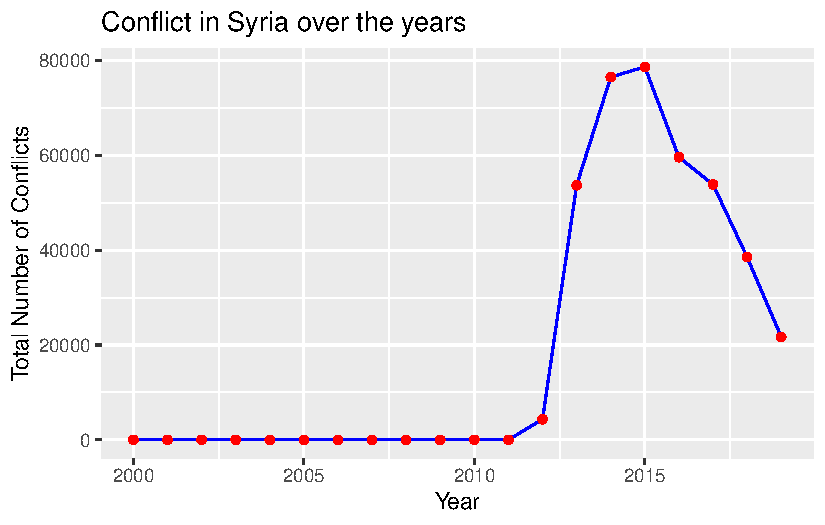
\includegraphics{armed_conflict_eda_files/figure-pdf/unnamed-chunk-7-1.pdf}

\begin{Shaded}
\begin{Highlighting}[]
\CommentTok{\# Reshape the data to long format}
\NormalTok{syria }\OtherTok{=} \FunctionTok{subset}\NormalTok{(finaldata, country\_name }\SpecialCharTok{==} \StringTok{"Syria"}\NormalTok{)}
\NormalTok{data\_long }\OtherTok{\textless{}{-}}\NormalTok{ syria }\SpecialCharTok{\%\textgreater{}\%}
  \FunctionTok{pivot\_longer}\NormalTok{(}\AttributeTok{cols =} \FunctionTok{c}\NormalTok{(MatMor, InfMor, Und5Mor, NeoMor), }
               \AttributeTok{names\_to =} \StringTok{"MortalityType"}\NormalTok{, }
               \AttributeTok{values\_to =} \StringTok{"Rate"}\NormalTok{)}

\CommentTok{\# Create the plot}
\FunctionTok{ggplot}\NormalTok{(data\_long, }\FunctionTok{aes}\NormalTok{(}\AttributeTok{x =}\NormalTok{ year, }\AttributeTok{y =}\NormalTok{ Rate, }\AttributeTok{color =}\NormalTok{ MortalityType)) }\SpecialCharTok{+}
      \FunctionTok{geom\_line}\NormalTok{() }\SpecialCharTok{+}
      \FunctionTok{geom\_point}\NormalTok{() }\SpecialCharTok{+} 
      \FunctionTok{labs}\NormalTok{(}\AttributeTok{title =} \StringTok{"Mortality Rates in Syria over the years"}\NormalTok{, }
           \AttributeTok{x =} \StringTok{"Year"}\NormalTok{, }
           \AttributeTok{y =} \StringTok{"Mortality Rate"}\NormalTok{) }\SpecialCharTok{+}
      \FunctionTok{scale\_color\_manual}\NormalTok{(}\AttributeTok{values =} \FunctionTok{c}\NormalTok{(}\StringTok{"MatMor"} \OtherTok{=} \StringTok{"blue"}\NormalTok{, }
                                      \StringTok{"InfMor"} \OtherTok{=} \StringTok{"red"}\NormalTok{, }
                                      \StringTok{"Und5Mor"} \OtherTok{=} \StringTok{"green"}\NormalTok{, }
                                      \StringTok{"NeoMor"} \OtherTok{=} \StringTok{"orange"}\NormalTok{))}
\end{Highlighting}
\end{Shaded}

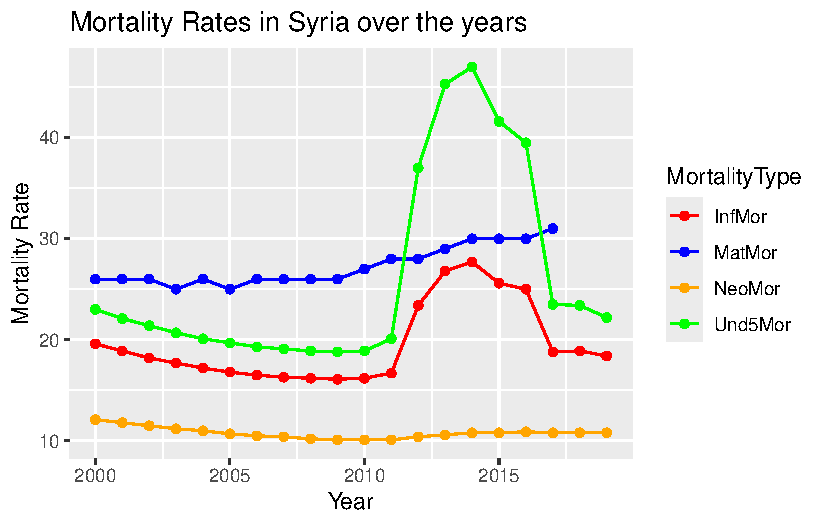
\includegraphics{armed_conflict_eda_files/figure-pdf/unnamed-chunk-7-2.pdf}

These two plots align with each other in the fact that their maximums
occur around 2015, which is expected. When there was a higher number of
conflicts, the mortality rates (perhaps excluding neonatal) also
obtained their max values in Syria.




\end{document}
